\documentclass[CJK]{ctexart}
\usepackage{CJK}
\usepackage{color}
\usepackage{amsmath}
\usepackage{listings}
\usepackage[framed,numbered,autolinebreaks,useliterate]{mcode}
\usepackage{textcomp}
\CTEXsetup[format={\Large\bfseries}]{section}
\usepackage{graphicx}
\usepackage{subfigure}
\usepackage{lastpage}
\usepackage{float}
\usepackage[superscript]{cite}
\usepackage{geometry}
\usepackage{bm}

\geometry{left=3cm,right=3cm,top=1.5cm,bottom=1.5cm}

\begin{document}
\title{\textbf{混合高斯分布相关问题的讨论}}
\author{518021910677 朱展达}
\date{Dec. 10th, 2019}
\maketitle

\section{问题说明}

\textbf{混合高斯分布}:$X\sim N(\mu_1, \sigma_1^2)$,$Y\sim N(\mu_2,\sigma_2^2)$,变量$\eta$满足二项分布。则称$Z=X+\eta Y$服从的分布为混合高斯分布。其中,$\eta$服从的二项分布如下表:
    \begin{table}[h]
        \caption{$\eta$ 分布列}
        \begin{center}
        \begin{tabular}{|c|c|c|}
        \hline
        $ \eta $ & $ 0 $     & $ 1 $ \\
        \hline
        $ P $    & $ 1 - p $ & $ p $ \\
        \hline
        \end{tabular}
        \end{center}
    \end{table}

    \textbf{问题1:}
    \begin{itemize}
        \item 自己设定参数,用计算机生成10000个混合高斯分布的随机数;
        \item 画出其频率分布直方图;
        \item 讨论不同参数对其分布“峰”的影响。
    \end{itemize}

    \textbf{问题2:}
    自己设定参数,用计算机生成1000组,每组$n$个混合高斯分布的随机数。第$i$组随机数记为:$Z_{i,1},Z_{i,2}, ... ,Z_{i,n}$,$i = 1, 2, ..., 1000$。
    定义
    \begin{equation}
        U_i = \frac{\sum_{j=1}^n{Z_{i, j}} - nEZ}{\sqrt{nDZ}}
        \label{equation1}
    \end{equation}
    \begin{itemize}
        \item 画出$U_1,U_2,...,U_{1000}$的频率分布直方图;
        \item 讨论不同$n=10,20,50,100,1000$对频率直方图“峰”的影响;
        \item 你能从中得到什么结论?
    \end{itemize}

\section{问题分析、求解思路与代码}

\subsection{问题分析}

问题1主要是探索混合高斯分布,根据其形式,其应为两个正态分布的加权平均,需要考虑$\mu_1,\sigma_1,\mu_2,\sigma_2,p$对峰的影响;问题2主要是利用混合高斯分布来探索验证 Lindeberg-L\'{e}vy 中心极限定理。

\subsection{问题1求解思路与代码}

通过matlab生成相应混合高斯分布,利用hist和bar函数生成相应的频率分布直方图,通过固定其中四个参数,多次改变另一个参数,来分析其对峰的影响。代码如下:


\lstinputlisting{solution_for_problem1.m}

\subsection{问题2求解思路与代码}

由于式(1)中$EZ$和$DZ$为理论值,先计算混合高斯分布$Z$的均值和方差:

\begin{equation}
    EZ = E(X+\eta Y) = EX+E\eta \cdot EY = \mu_1 + p\mu_2
\end{equation}

\begin{equation}
    \begin{aligned}
        EZ^2 &= E((X+\eta Y)^2) = E(X^2 + 2\eta XY + \eta^2 Y^2) \\
             &= EX^2 + 2(EX)(EY)(E\eta) + E(\eta^2)E(Y^2) \\
             &= \mu_1^2 + \sigma_1^2 + 2\mu_1 \mu_2 p + (\mu_2^2 + \sigma_2^2) p   
    \end{aligned}
\end{equation}

\begin{equation}
    \begin{aligned}
        DZ &= EZ^2 - (EZ)^2 = \sigma_1^2 + p \sigma_2^2 + p(1-p)\mu_2^2
    \end{aligned}
\end{equation}

确定合适的参数,生成1000组混合高斯分布的随机数,分别计算$U_i$,$i=1,2,...,1000$。做$n=10,20,50,100,1000$的图进行比较讨论。

由于$EZ$和$DZ$在$(\mu_1, \sigma_1,\mu_2,\sigma_2,p)$确定时是常量,由 Lindeberg-L\'{e}vy 中心极限定理知,当$n$足够大时,$U_i$服从标准正态分布。为了使图像随着$n$的改变变化明显,要尽量破坏原分布的正态分布性,因为对于$Z$分布得到的频率直方图的两个“峰”,当$\sigma$较小时,取值分布在“峰”两边。因此令$|\mu_2|$很大时,$x$取值在两峰之间的概率很小,可以破坏原有的正态分布性。

代码如下:

\lstinputlisting{solution_for_problem2.m}

\section{问题1求解}

\subsection{讨论$\mu_1$对分布“峰”的影响}

固定参数$\sigma_1=2,\mu_2=15,\sigma_2=3,p=0.7$,改变$\mu$取值,令$\mu_1$分别为$0,4,8,12,16,20$,观察得到的频率分布直方图。

\begin{figure}[H]
    \centering
    \subfigure[$\mu_1 = 0$]{
    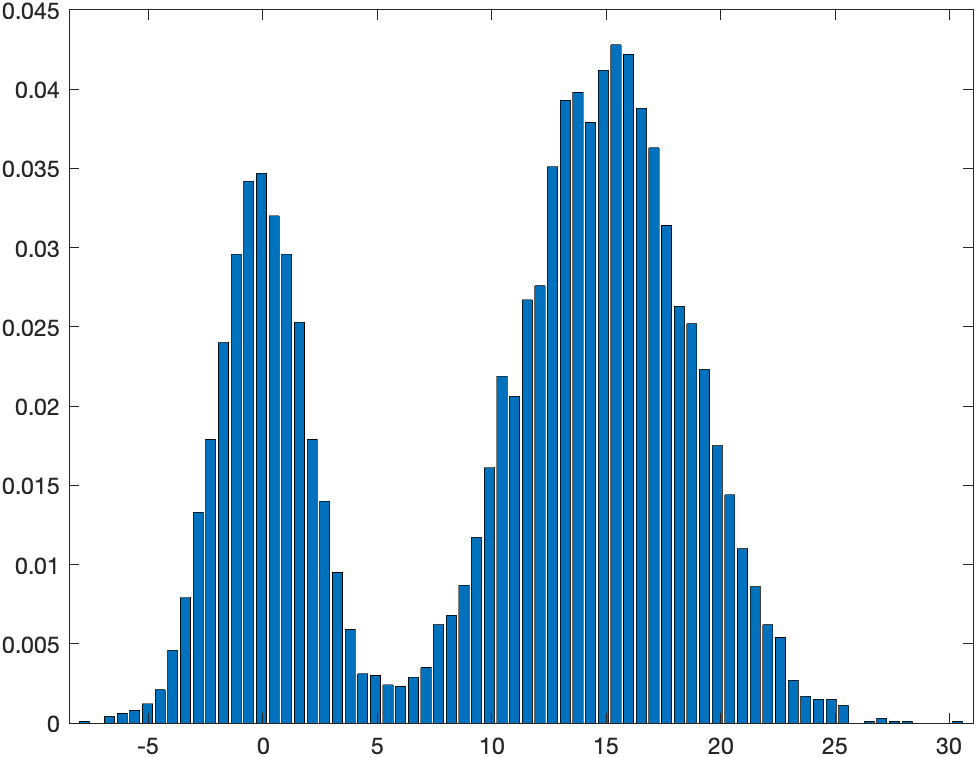
\includegraphics[width=4.3cm]{1-1.png}
    %\caption{fig1}
    }
    \quad
    \subfigure[$\mu_1 = 4$]{
    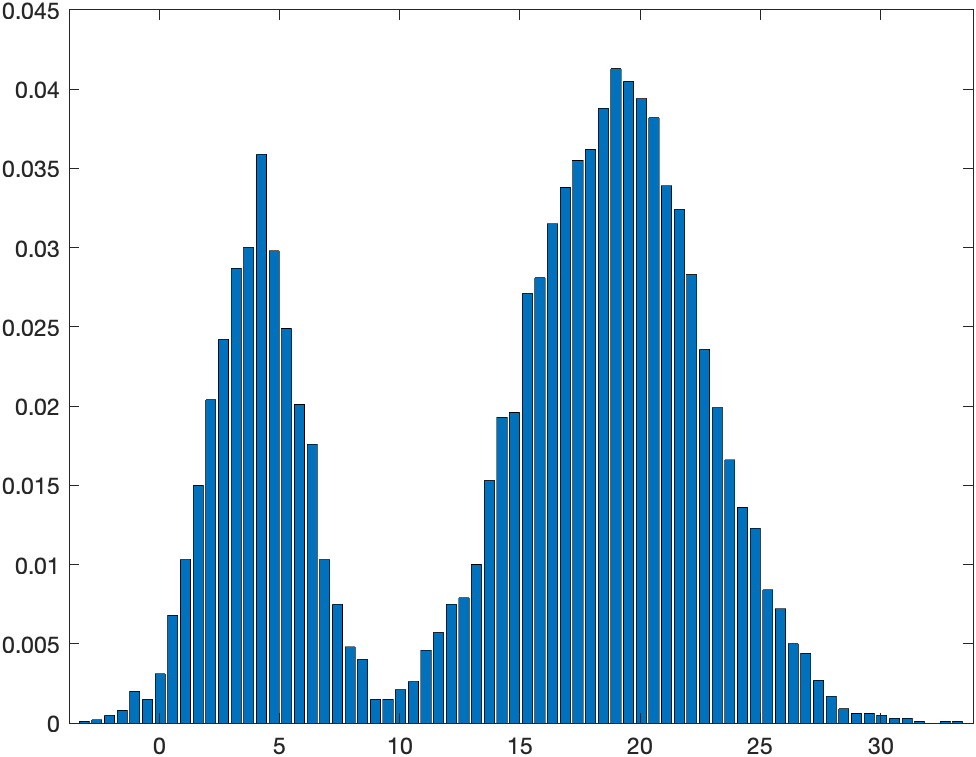
\includegraphics[width=4.3cm]{1-2.png}
    %\caption{fig1}
    }
    \quad
    \subfigure[$\mu_1 = 8$]{
    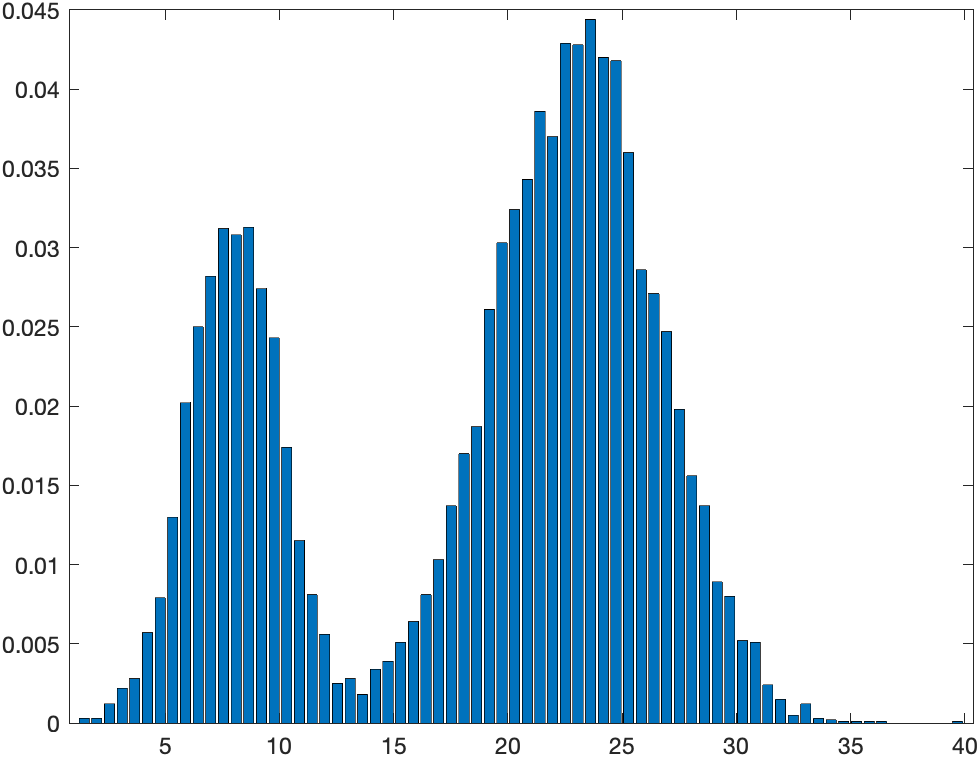
\includegraphics[width=4.3cm]{1-3.png}
    }
    \quad
    \subfigure[$\mu_1 = 12$]{
    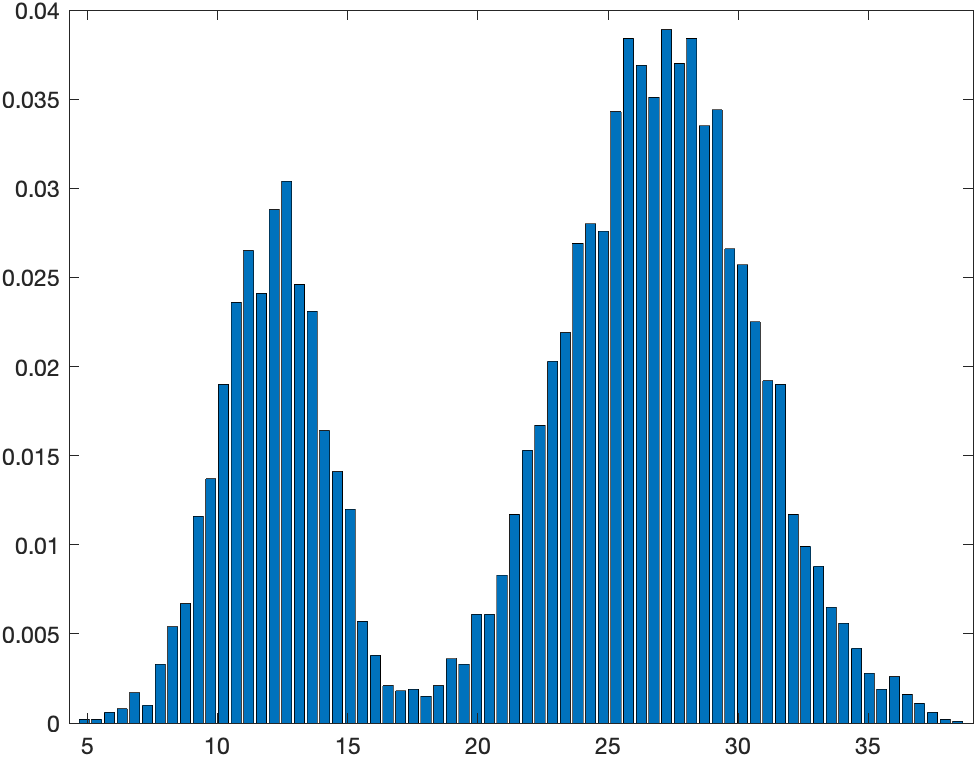
\includegraphics[width=4.3cm]{1-4.png}
    }
    \quad
    \subfigure[$\mu_1 = 16$]{
    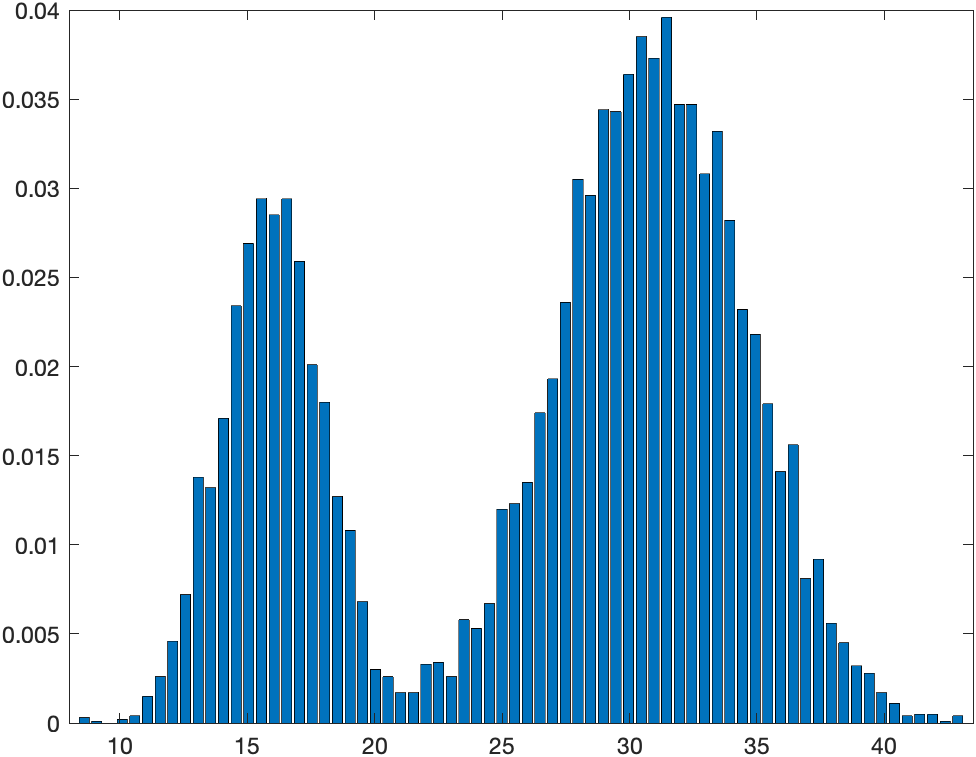
\includegraphics[width=4.3cm]{1-5.png}
    }
    \quad
    \subfigure[$\mu_1 = 20$]{
    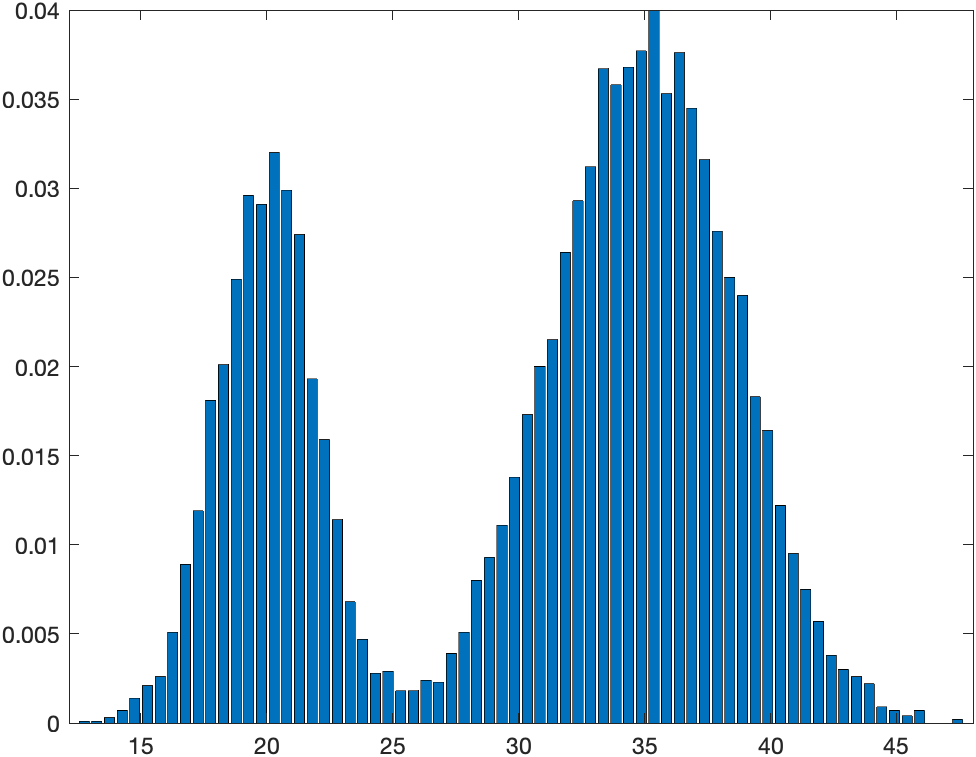
\includegraphics[width=4.3cm]{1-6.png}
    }
    \caption{$\sigma_1=2,\mu_2=15,\sigma_2=3,p=0.7$下,$\mu_1$变化时生成的随机数的频率分布直方图}
    \label{fig1}
\end{figure}

\textbf{结论:}从上述六图中我们可以发现,在$\mu_1$改变时,随机数的频率分布直方图的形态基本保持不变,整体图像仅随$\mu_1$的变化而平移。其中,第一个峰对应的$x$坐标为$\mu_1$,第二个峰对应的$x$坐标为$\mu_1+\mu_2$。

\subsection{讨论$\sigma_1$对分布“峰”的影响}

固定参数$\mu_1=0,\mu_2=15,\sigma_2=3,p=0.7$,改变$\sigma_1$取值,令$\sigma_1$分别为$1,2,4,6,10,20$,观察得到的频率分布直方图。

\begin{figure}[H]
    \centering
    \subfigure[$\sigma_1 = 1$]{
    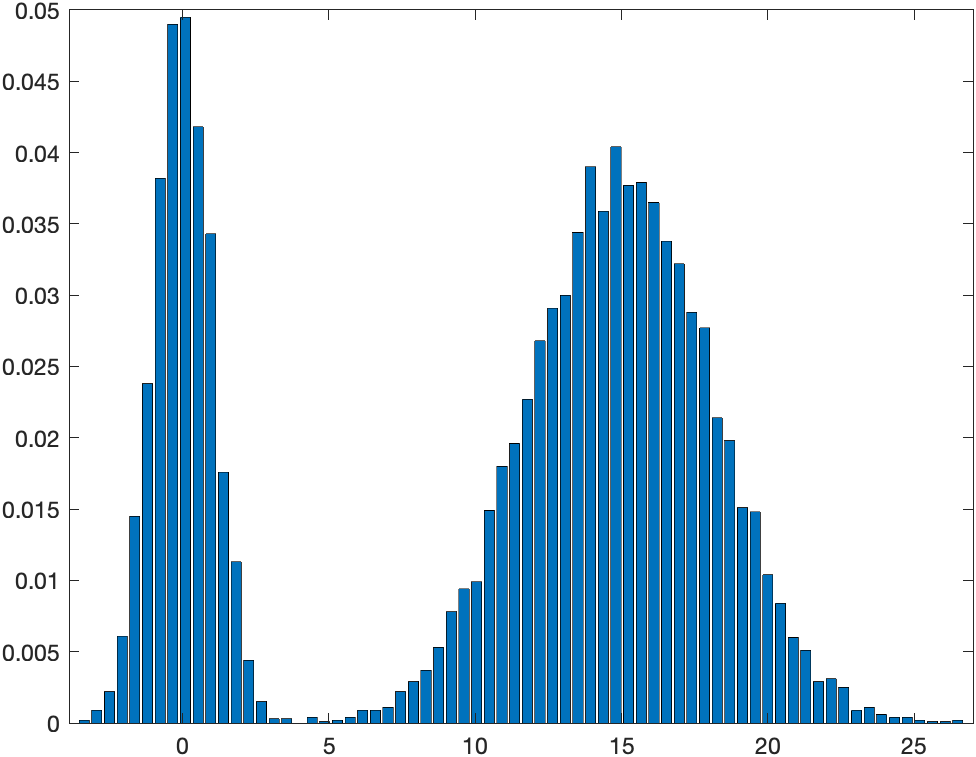
\includegraphics[width=4.3cm]{2-1.png}
    %\caption{fig1}
    }
    \quad
    \subfigure[$\sigma_1 = 2$]{
    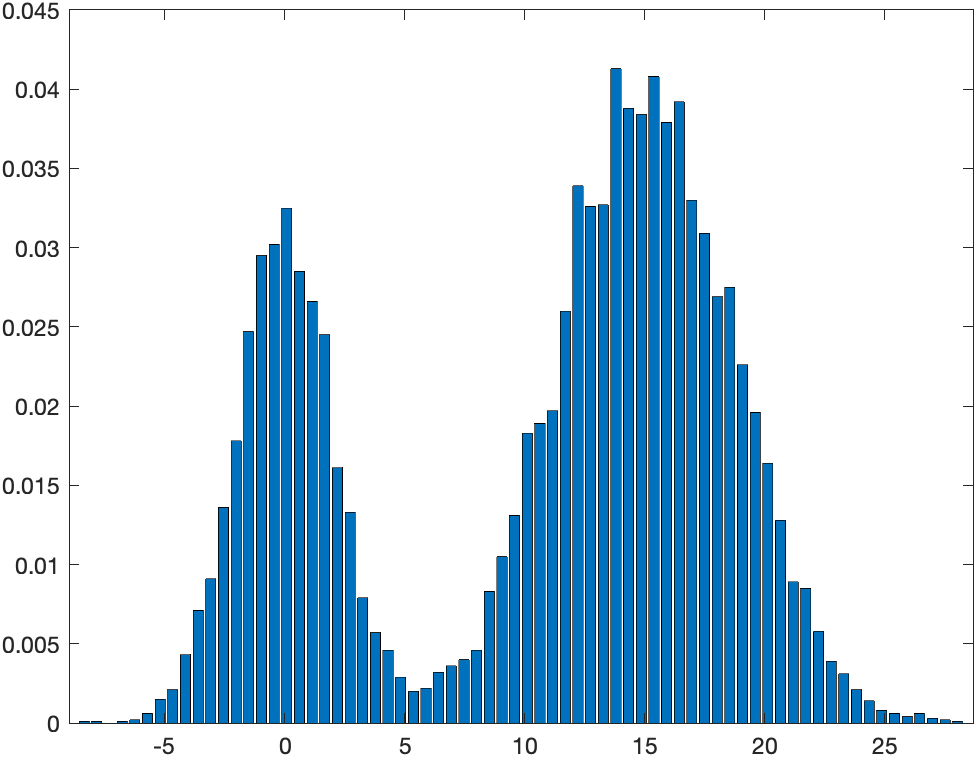
\includegraphics[width=4.3cm]{2-2.png}
    %\caption{fig1}
    }
    \quad
    \subfigure[$\sigma_1 = 4$]{
    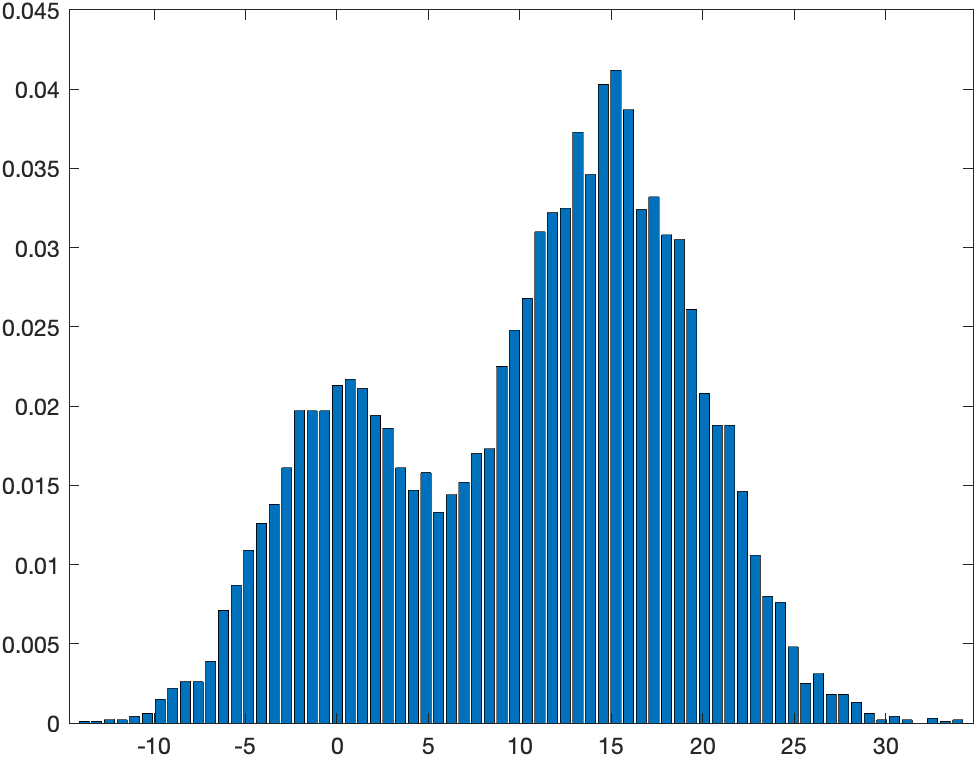
\includegraphics[width=4.3cm]{2-3.png}
    }
    \quad
    \subfigure[$\sigma_1 = 6$]{
    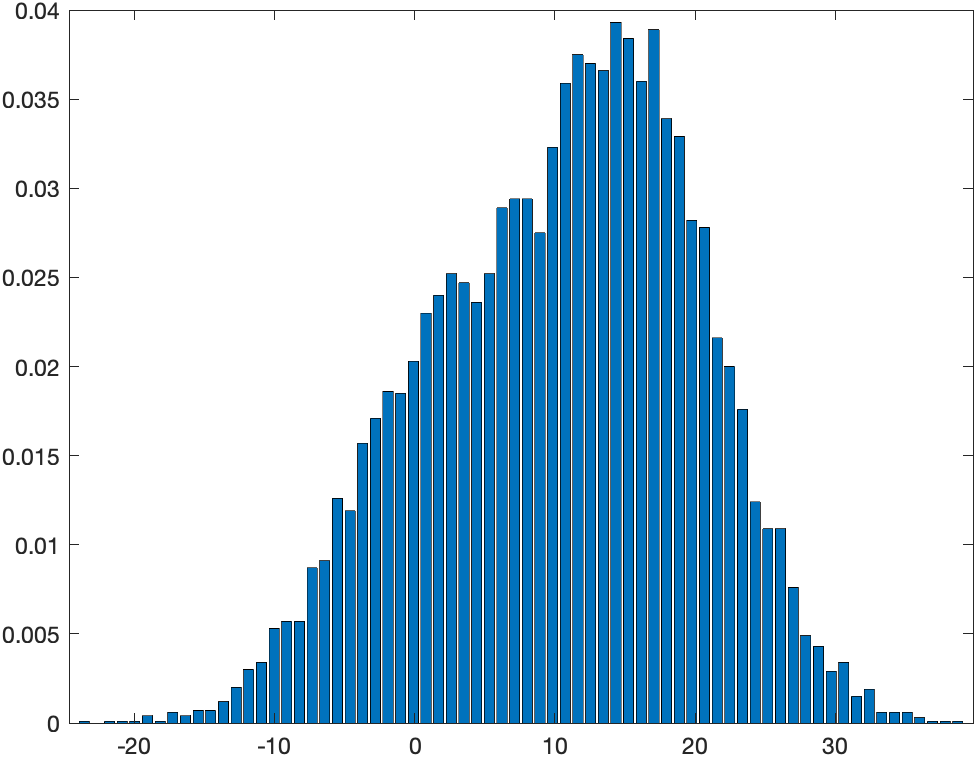
\includegraphics[width=4.3cm]{2-4.png}
    }
    \quad
    \subfigure[$\sigma_1 = 10$]{
    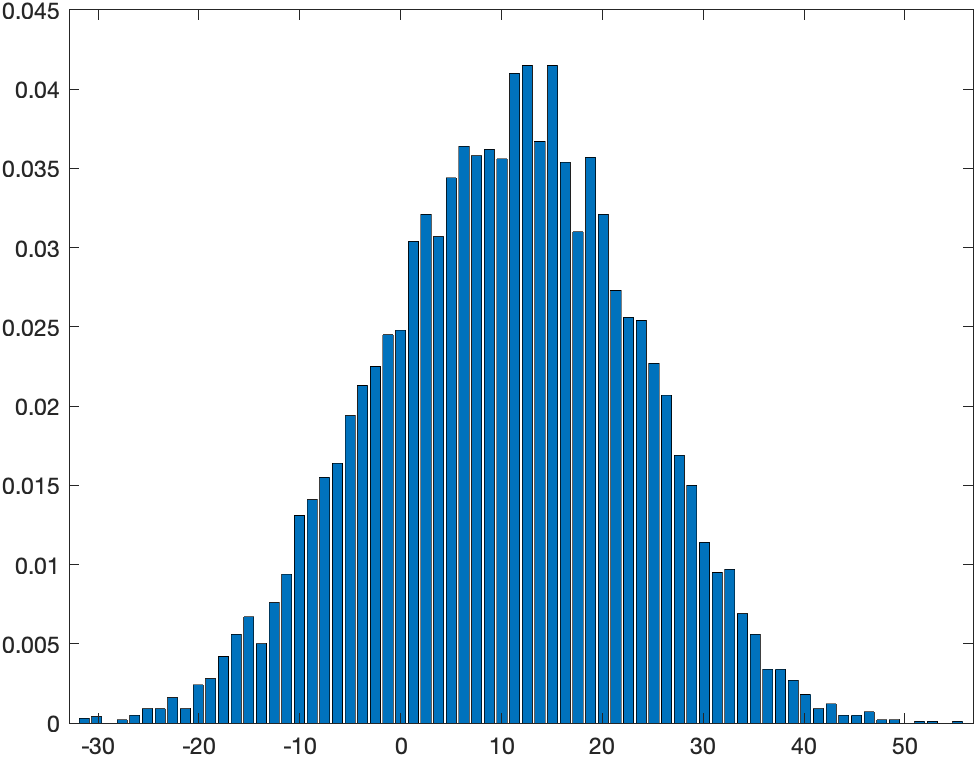
\includegraphics[width=4.3cm]{2-5.png}
    }
    \quad
    \subfigure[$\sigma_1 = 20$]{
    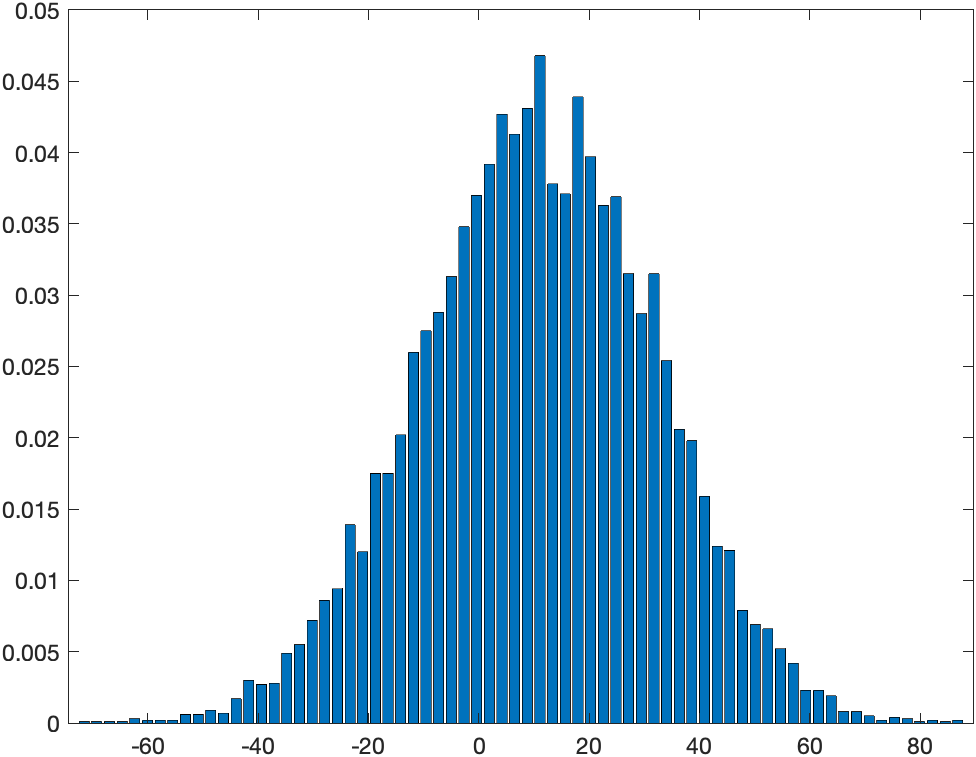
\includegraphics[width=4.3cm]{2-6.png}
    }
    \caption{$\mu_1=0,\mu_2=15,\sigma_2=3,p=0.7$下,$\sigma_1$变化时生成的随机数的频率分布直方图}
    \label{fig2}
\end{figure}

\textbf{结论:}从上述六图中我们可以发现,在$\sigma_1$变化时,“峰”的分布、数量、高度和峰两侧对应的斜率都会产生变化。当$\mu_2$不为0时,$\sigma_1$较小时会出两个“峰”,$\sigma_1$较大时两个“峰”会合并成一个“峰”。随着$\sigma_1$的增大,$\mu_1$对应的“峰”高度下降并且变得逐渐趋于平缓,$\mu_1+\mu_2$对应的“峰”高度有所升高,最终会产生两峰合并,只留下$\mu_1+\mu_2$对应的峰的情况。

\subsection{讨论$\mu_2$对分布“峰”的影响}

固定参数$\mu_1=0,\sigma_1=2,\sigma_2=3,p=0.7$,改变$\mu_2$取值,令$\mu_2$分别为$-10,-5,0,5,10,20$,观察得到的频率分布直方图。

\begin{figure}[H]
    \centering
    \subfigure[$\mu_2 = -10$]{
    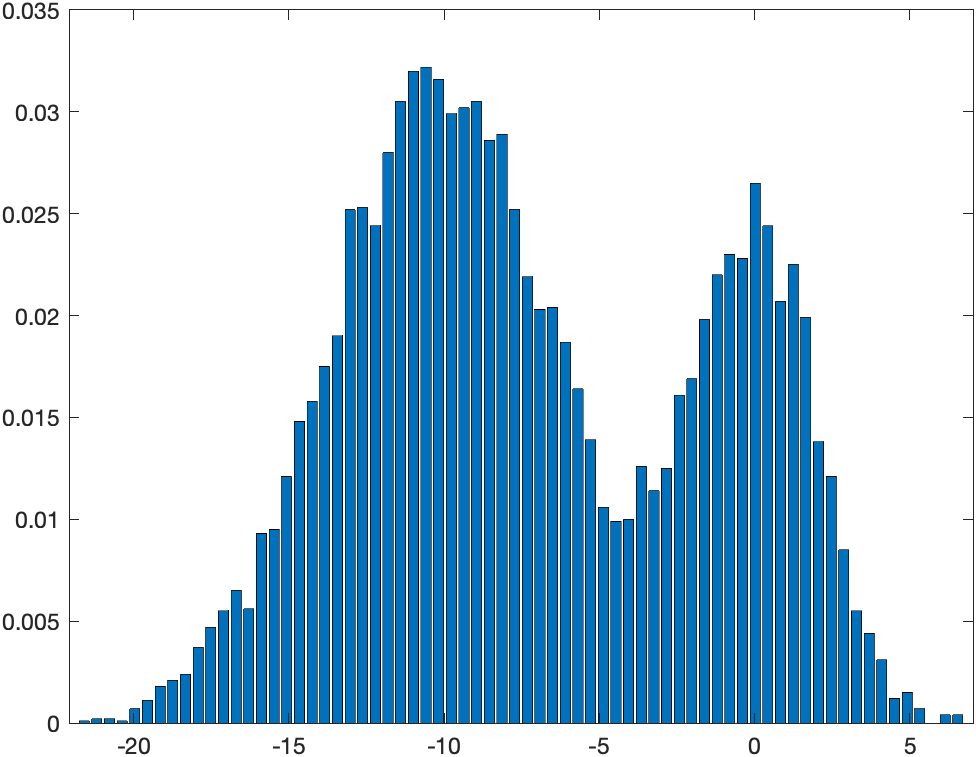
\includegraphics[width=4.3cm]{3-1.png}
    %\caption{fig1}
    }
    \quad
    \subfigure[$\mu_2 = -5$]{
    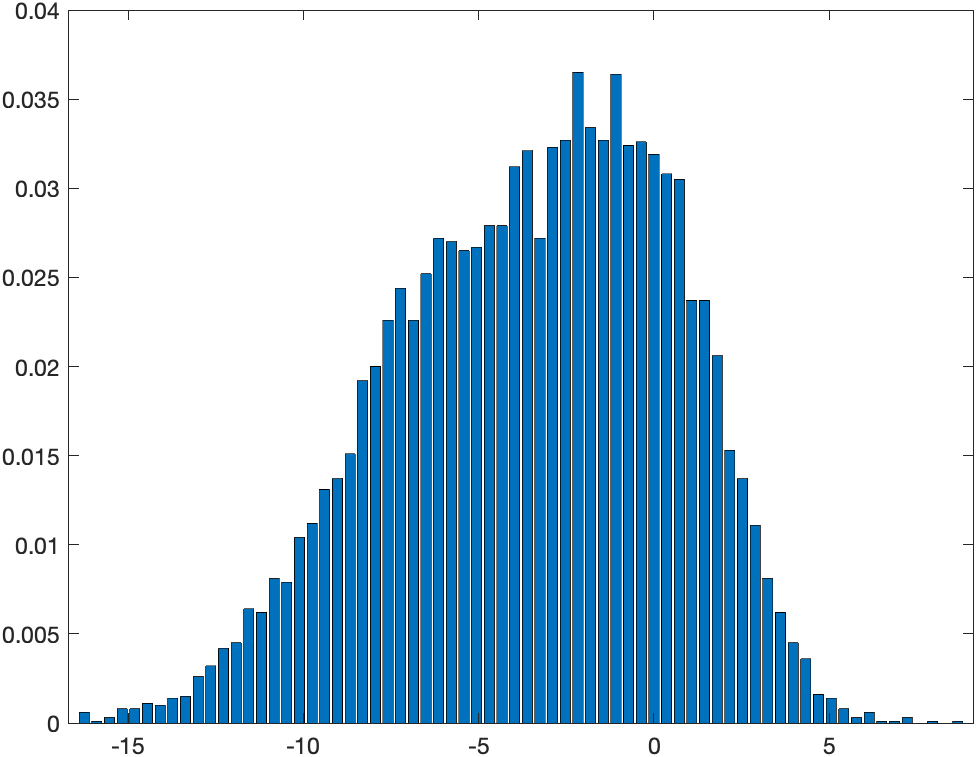
\includegraphics[width=4.3cm]{3-2.png}
    %\caption{fig1}
    }
    \quad
    \subfigure[$\mu_2 = 0$]{
    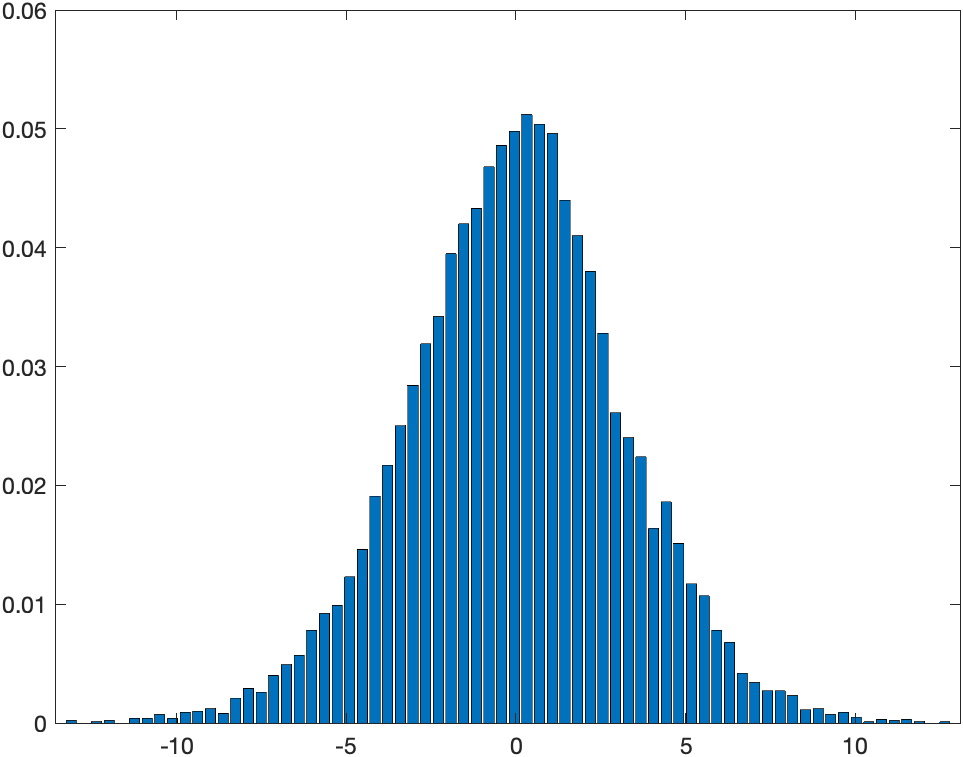
\includegraphics[width=4.3cm]{3-3.png}
    }
    \quad
    \subfigure[$\mu_2 = 5$]{
    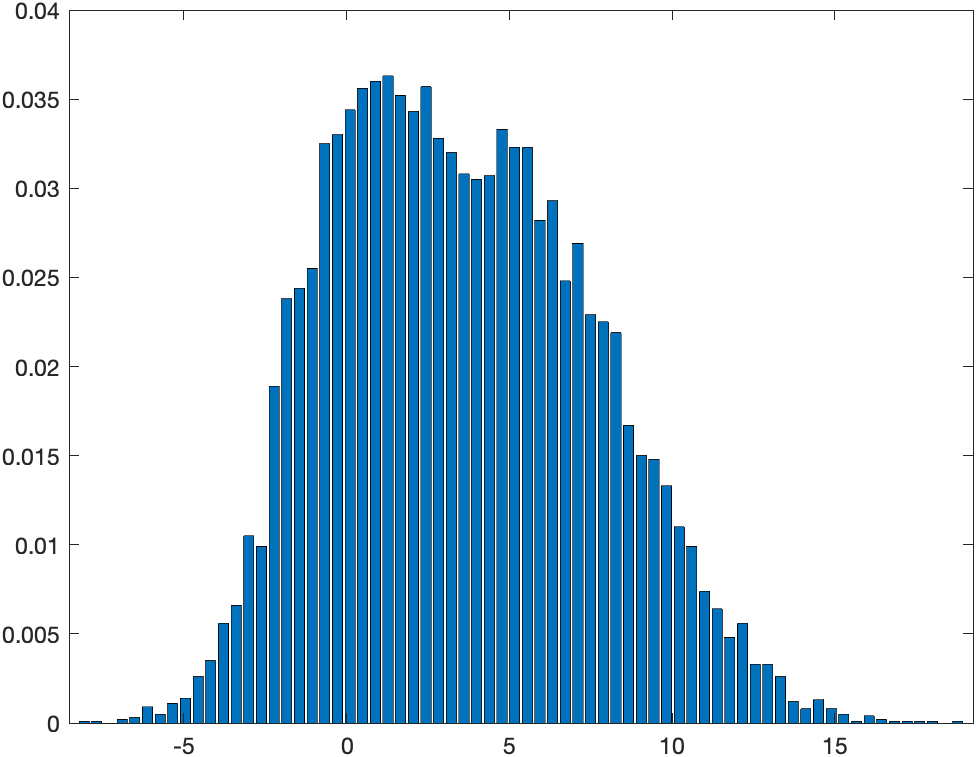
\includegraphics[width=4.3cm]{3-4.png}
    }
    \quad
    \subfigure[$\mu_2 = 10$]{
    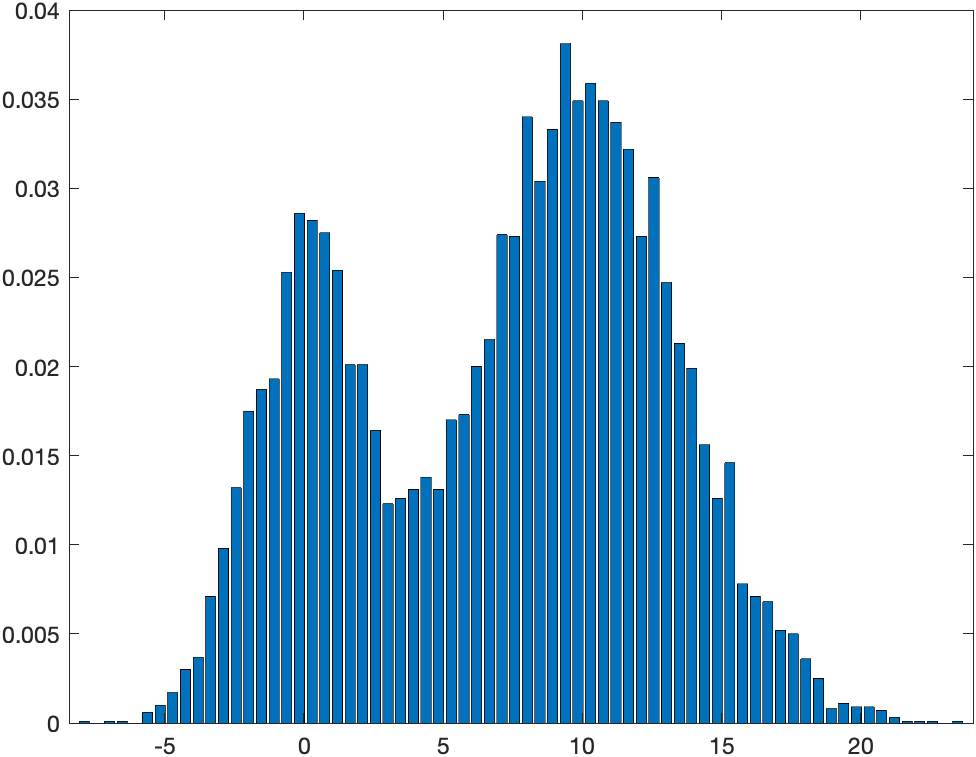
\includegraphics[width=4.3cm]{3-5.png}
    }
    \quad
    \subfigure[$\mu_2 = 20$]{
    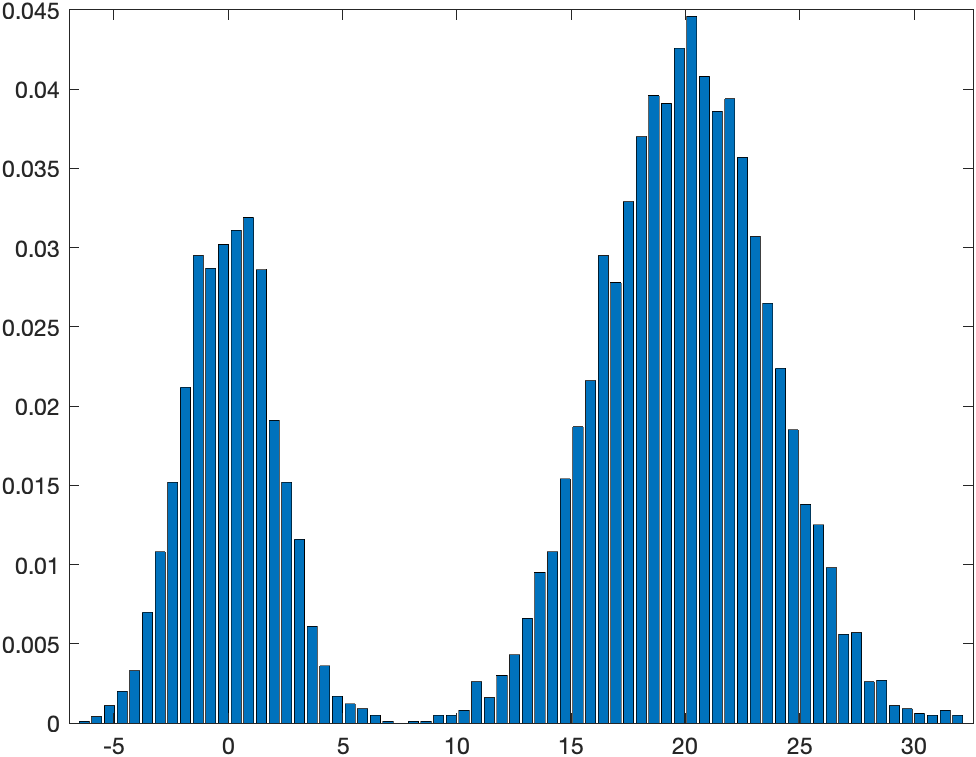
\includegraphics[width=4.3cm]{3-6.png}
    }
    \caption{$\mu_1=0,\sigma_1=2,\sigma_2=3,p=0.7$下,$\mu_2$变化时生成的随机数的频率分布直方图}
    \label{fig3}
\end{figure}

\textbf{结论:}从上述六图中我们可以发现,在$\mu_2$变化时,“峰”的数量和分布会发生变化。其中一个“峰”对应的$x$坐标一直为$\mu_1$,另一个“峰”对应的$x$坐标$\mu_1+\mu_2$会发生改变。当$|\mu_2|$较大时,有明显的两个“峰”,当$|\mu_2|$较小时,两座峰逐渐融合,当$\mu_2=0$时,完全只剩下一个“峰”。同时显然的,$\mu_2$的正负会影响两座峰的左右排布。

\subsection{讨论$\sigma_2$对分布“峰”的影响}

固定参数$\mu_1=0,\sigma_1=2,\mu_2=15,p=0.7$,改变$\sigma_2$取值,令$\sigma_1$分别为$1,2,4,6,10,20$,观察得到的频率分布直方图。

\begin{figure}[H]
    \centering
    \subfigure[$\sigma_2 = 1$]{
    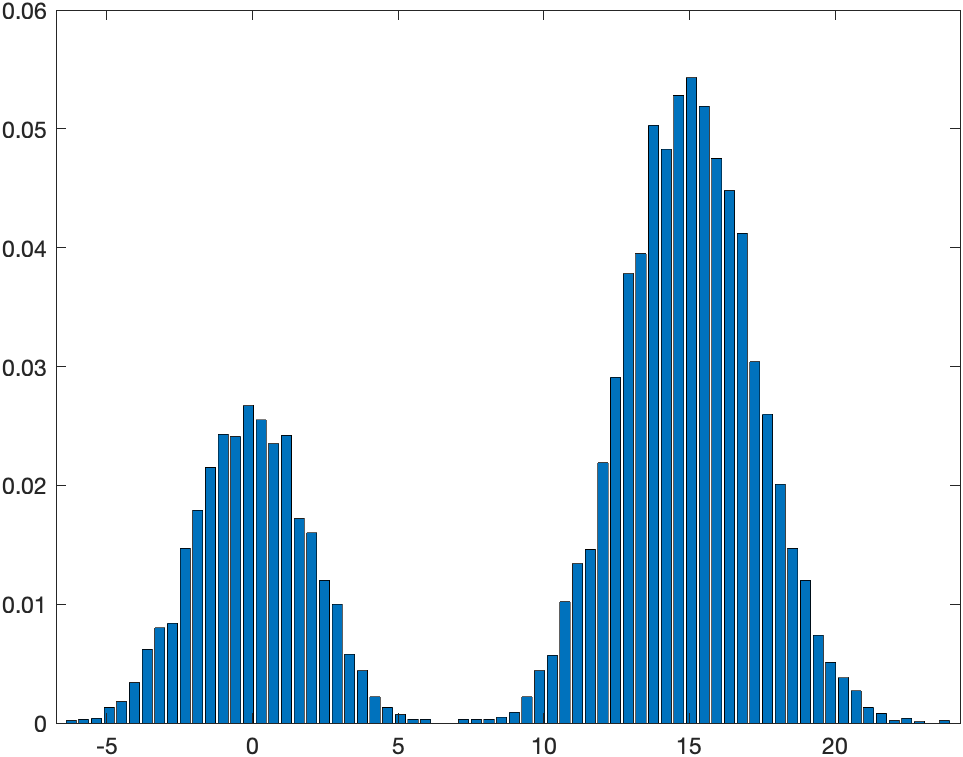
\includegraphics[width=4.3cm]{4-1.png}
    %\caption{fig1}
    }
    \quad
    \subfigure[$\sigma_2 = 2$]{
    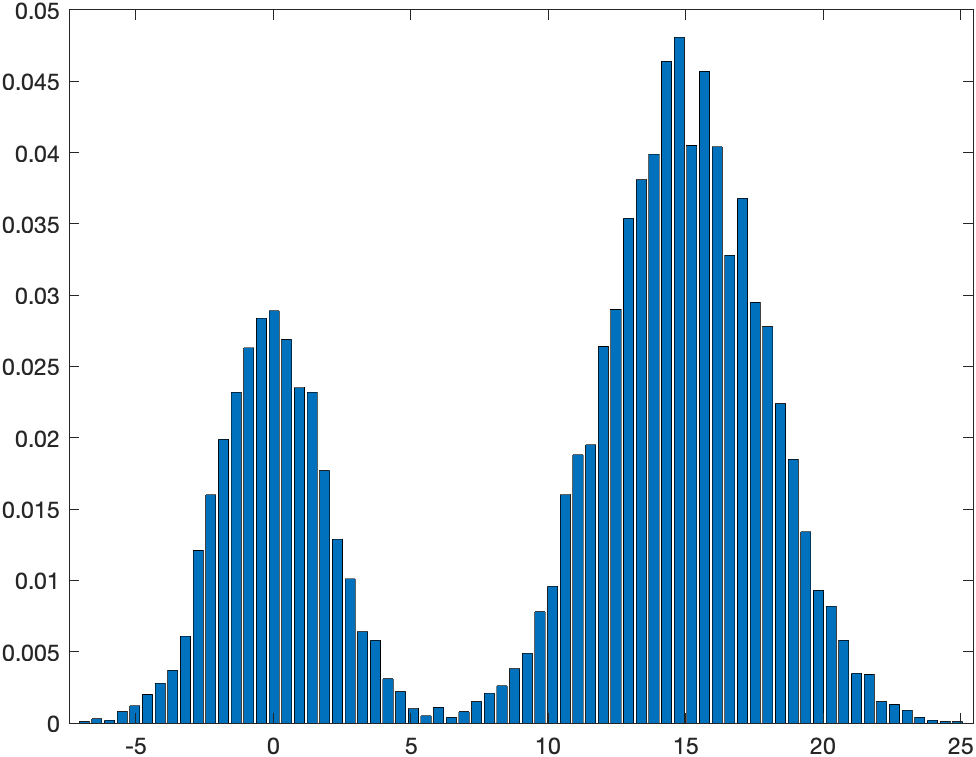
\includegraphics[width=4.3cm]{4-2.png}
    %\caption{fig1}
    }
    \quad
    \subfigure[$\sigma_2 = 4$]{
    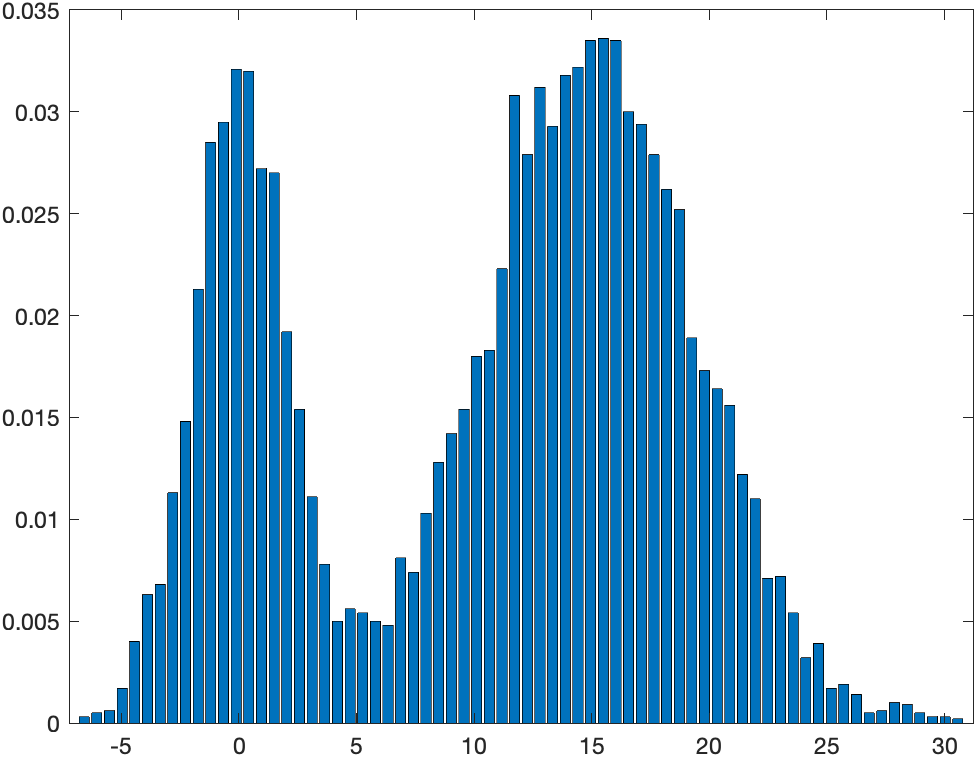
\includegraphics[width=4.3cm]{4-3.png}
    }
    \quad
    \subfigure[$\sigma_2 = 6$]{
    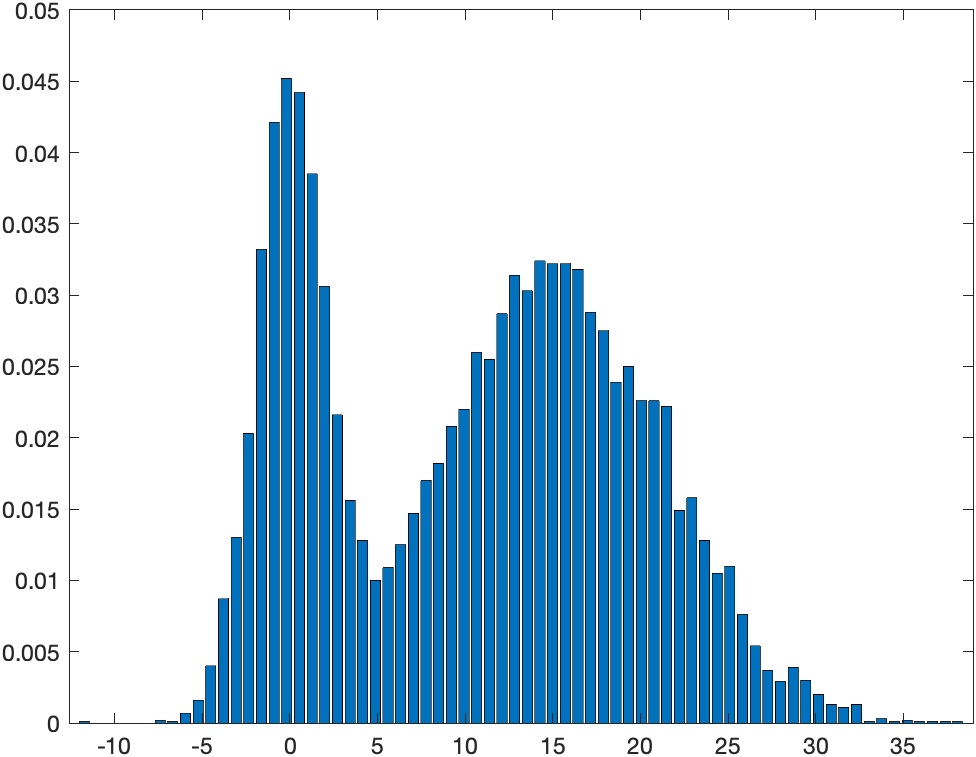
\includegraphics[width=4.3cm]{4-4.png}
    }
    \quad
    \subfigure[$\sigma_2 = 10$]{
    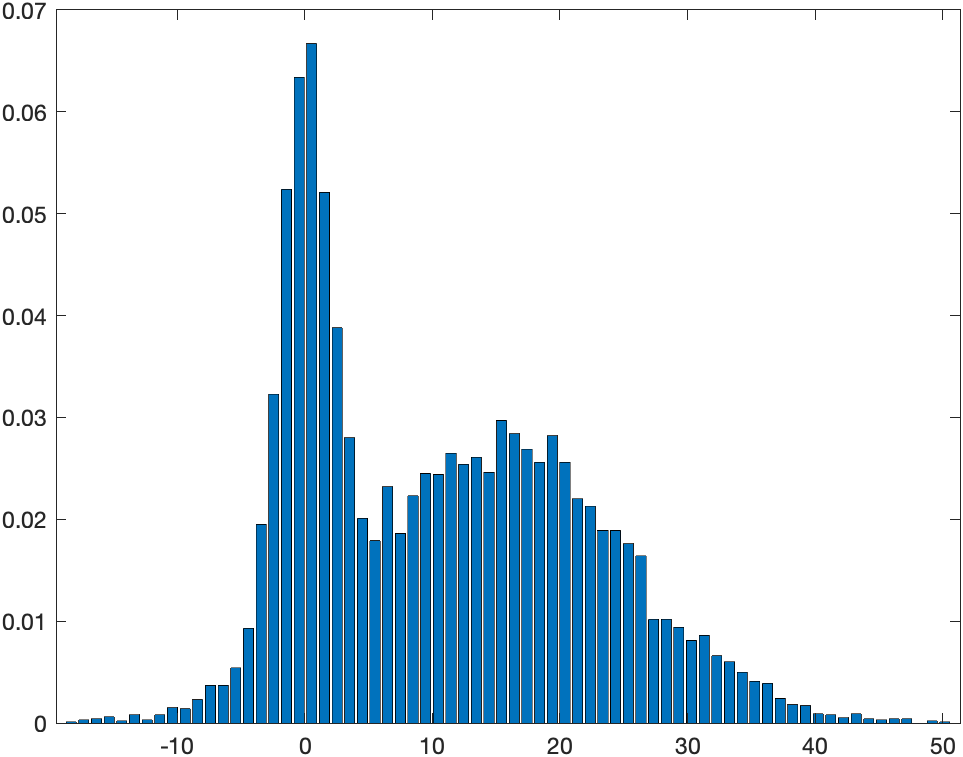
\includegraphics[width=4.3cm]{4-5.png}
    }
    \quad
    \subfigure[$\sigma_2 = 20$]{
    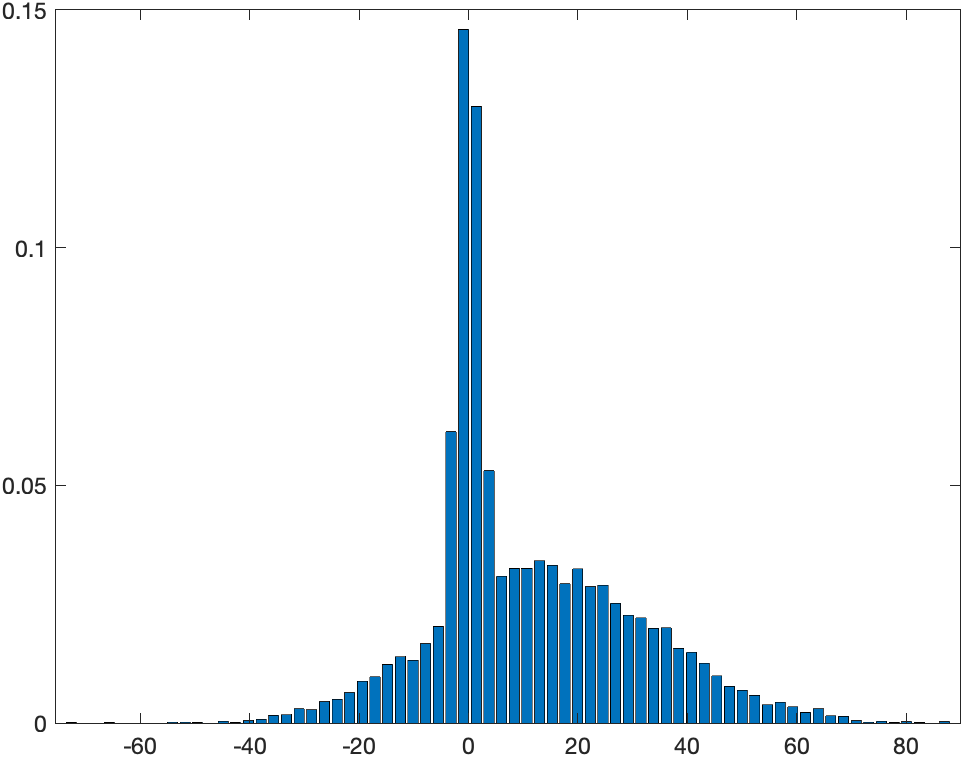
\includegraphics[width=4.3cm]{4-6.png}
    }
    \caption{$\mu_1=0,\sigma_1=2,\mu_2=15,p=0.7$下,$\sigma_2$变化时生成的随机数的频率分布直方图}
    \label{fig4}
\end{figure}

\textbf{结论:}从上述六图中我们可以发现,在$\sigma_2$变化时,“峰”的相对高度会发生变化。随着$\sigma_2$的增大,$\mu_1$对应的峰的高度升高,$\mu_1+\mu_2$对应的峰的高度下降,$\mu_1$对应的峰与$\mu_1+\mu_2$对应的峰的相对高度的代数值增大。且特别地,当$\sigma_2$特别大时,$\mu_1+\mu_2$所对应的峰会趋于消失,只剩下$\mu_1$所对应的峰。

\subsection{讨论$p$对分布“峰”的影响}

固定参数$\mu_1=0,\sigma_1=2,\mu_2=15,\sigma_2=3$,改变$p$取值,令$p$分别为$0, 0.2, 0.4, 0.6, 0.8, 1.0$,观察得到的频率分布直方图。

\begin{figure}[H]
    \centering
    \subfigure[$p = 0$]{
    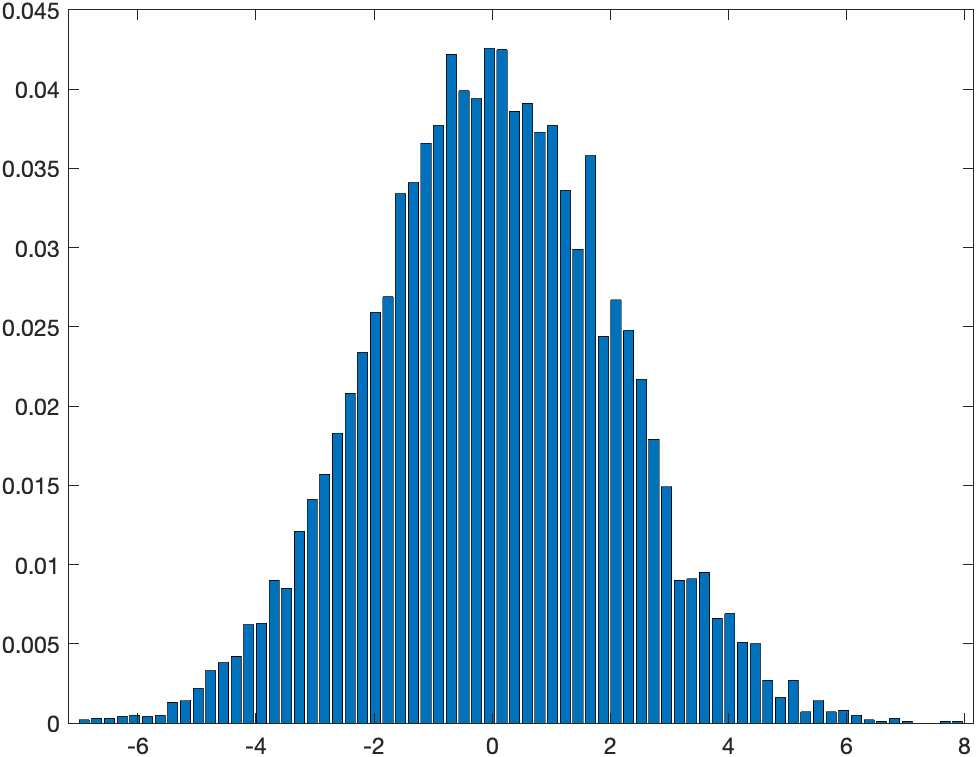
\includegraphics[width=4.3cm]{5-1.png}
    %\caption{fig1}
    }
    \quad
    \subfigure[$p = 0.2$]{
    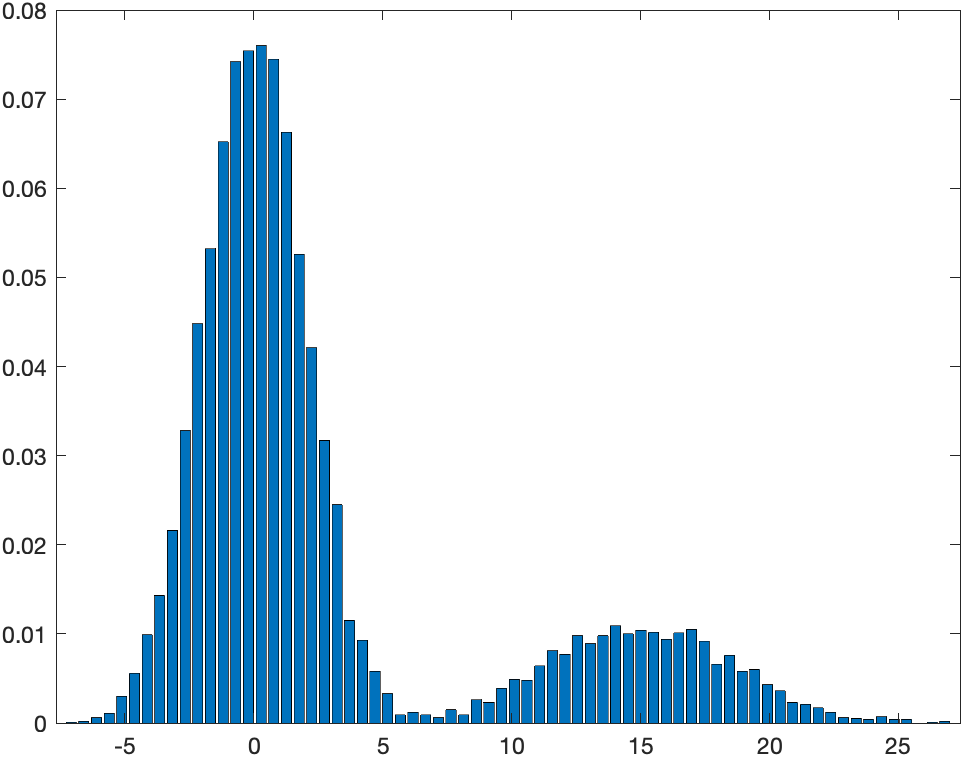
\includegraphics[width=4.3cm]{5-2.png}
    %\caption{fig1}
    }
    \quad
    \subfigure[$p = 0.4$]{
    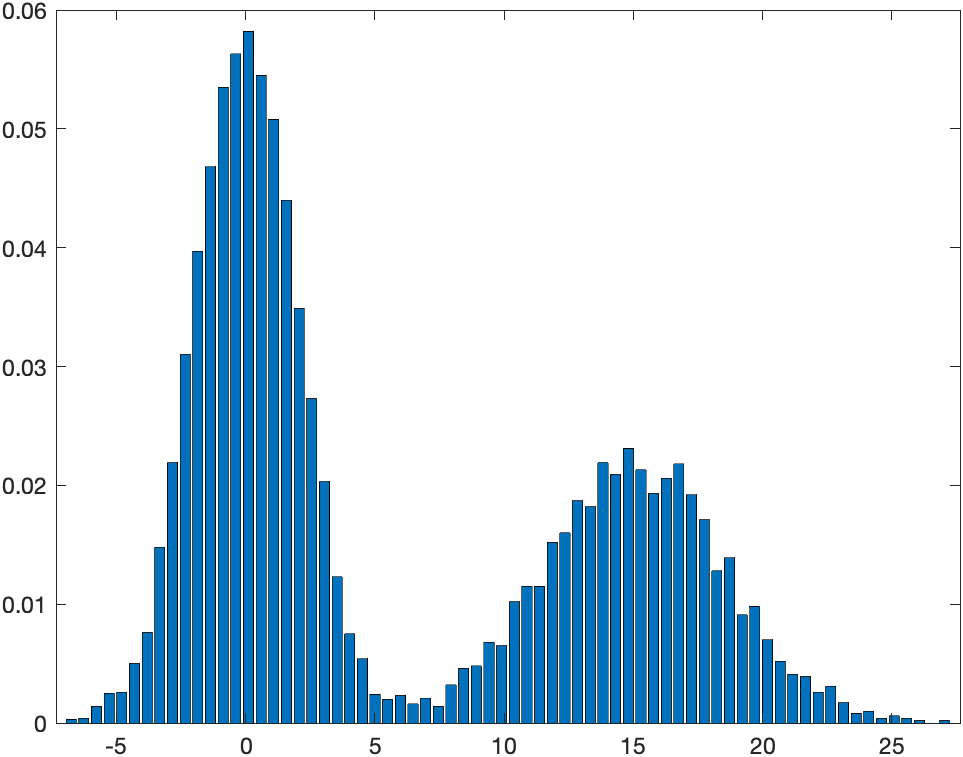
\includegraphics[width=4.3cm]{5-3.png}
    }
    \quad
    \subfigure[$p = 0.6$]{
    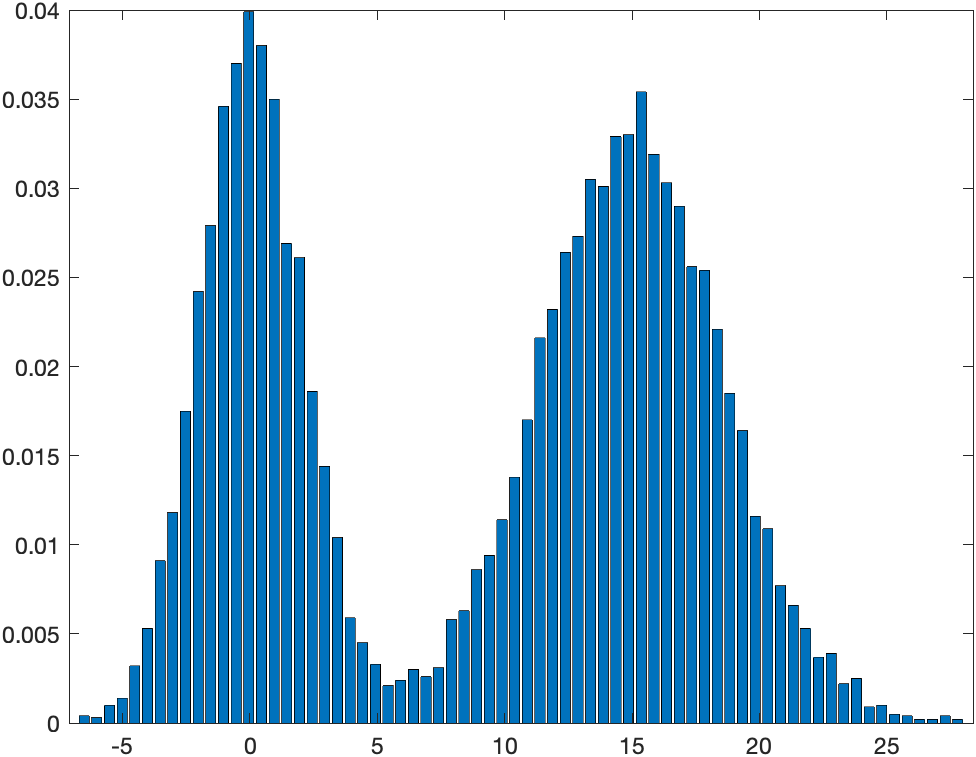
\includegraphics[width=4.3cm]{5-4.png}
    }
    \quad
    \subfigure[$p = 0.8$]{
    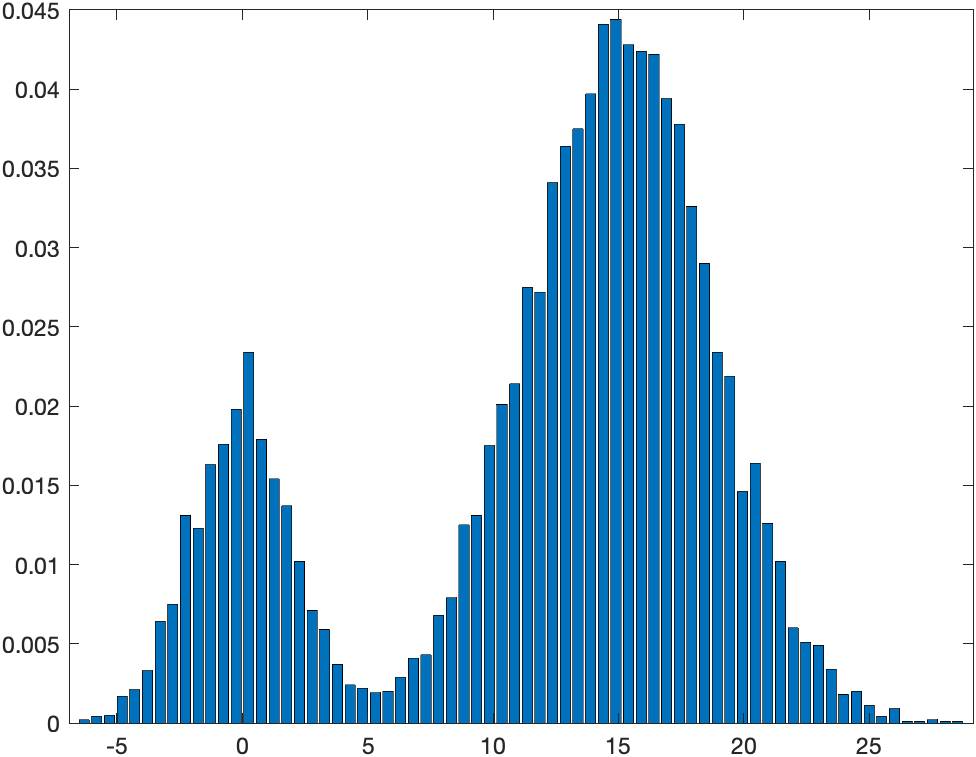
\includegraphics[width=4.3cm]{5-5.png}
    }
    \quad
    \subfigure[$p = 1.0$]{
    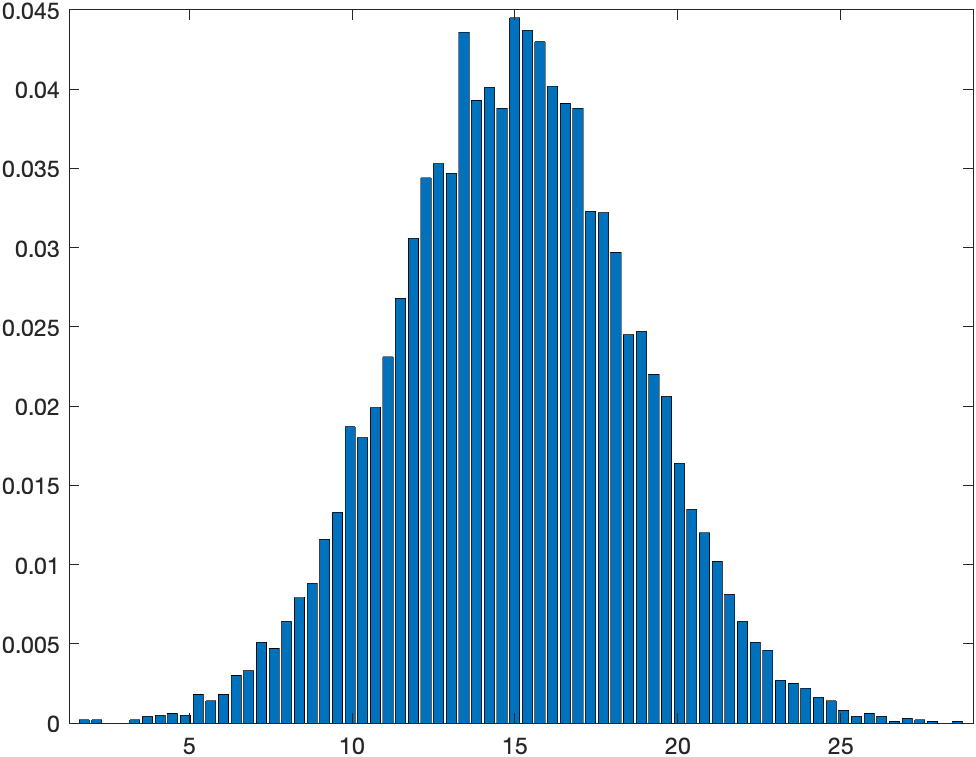
\includegraphics[width=4.3cm]{5-6.png}
    }
    \caption{$\mu_1=0,\sigma_1=2,\mu_2=15,\sigma_2=3$下,$p$变化时生成的随机数的频率分布直方图}
    \label{fig5}
\end{figure}

\textbf{结论:}从上述六图中我们可以发现,在$p$变化时,“峰”的数量、分布和高度会发生变化。$p=0$时,只有一个对应$x$坐标为$\mu_1$的“峰”;随着$p$的增大,$\mu_1$对应的“峰”的高度下降,$\mu_1+\mu_2$对应的“峰”的高度升高,$\mu_1$对应的“峰”与$\mu_1+\mu_2$对应的“峰”的相对高度的代数值降低;当$p=1$时,只剩下一个对应$x$坐标为$\mu_1+\mu_2$的峰。

\subsection{问题一结论总结与概括}

\begin{itemize}
    \item 混合高斯分布是两个正态分布的加权平均,每个正态分布单独存在时的频率分布直方图存在一个“峰”。故混合高斯分布得到的频率分布直方图存在两个“峰”,他们对应的$x$坐标分别为$\mu_1$,$\mu_1+\mu_2$,但这两个“峰”的位置、高度、平缓程度会受五个参数$(\mu_1,\sigma_1,\mu_2,\sigma_2,p)$的影响,有时两个峰变成只有一个峰。
    \item {
        \begin{enumerate}
            \item $\mu_1$会影响“峰”分布的$x$坐标,“峰”随$\mu_1$的变化而发生平移。
            \item $\sigma_1$会影响“峰”的数量、高度、平缓程度。随着$\sigma_1$的增大,$\mu_1$对应的“峰”高度下降并且变得逐渐趋于平缓,$\mu_1+\mu_2$对应的“峰”的高度升高;当$\sigma_1$极大时,只剩下$\mu_1+\mu_2$对应的“峰”。
            \item $\mu_2$会影响“峰”的数量和分布。$|\mu_2|$较大时,有明显的两个“峰”,$|\mu_2|$逐渐变小时,两座峰逐渐融合,当$\mu_2=0$时,只剩下一个“峰”。
            \item $\sigma_2$会影响“峰”的数量、高度、平缓程度。随着$\sigma_2$的增大,$\mu_1$对应的“峰”高度升高,$\mu_1+\mu_2$对应的“峰”高度下降并逐渐趋于平缓;当$\sigma_2$极大时,只剩下$\mu_1$对应的“峰”。
            \item $p$会影响“峰”的数量、分布和高度。$p=0$时,只有一个对应$x$坐标为$\mu_1$的“峰”;随着$p$的增大,$\mu_1$对应的“峰”的高度下降,$\mu_1+\mu_2$对应的“峰”的高度升高,$\mu_1$对应的“峰”与$\mu_1+\mu_2$对应的“峰”的相对高度的代数值降低;当$p=1$时,只剩下一个对应$x$坐标为$\mu_1+\mu_2$的峰。
        \end{enumerate}
    }   
\end{itemize}

\section{问题2求解}

\subsection{参数选择}

根据\textbf{2.3}的分析,需要让$|\mu_2|$值较大,取$\mu_1 = 0$,$ \sigma_1 = 2$,$ \mu_2 = 100$,$ \sigma_2 = 3$,$ p = 0.7$。

\subsection{频率直方图}

分别选择$n=10,20,50,100,1000$,得到相应的关系图。

\begin{figure}[H]
    \centering
    \subfigure[$n = 10$]{
    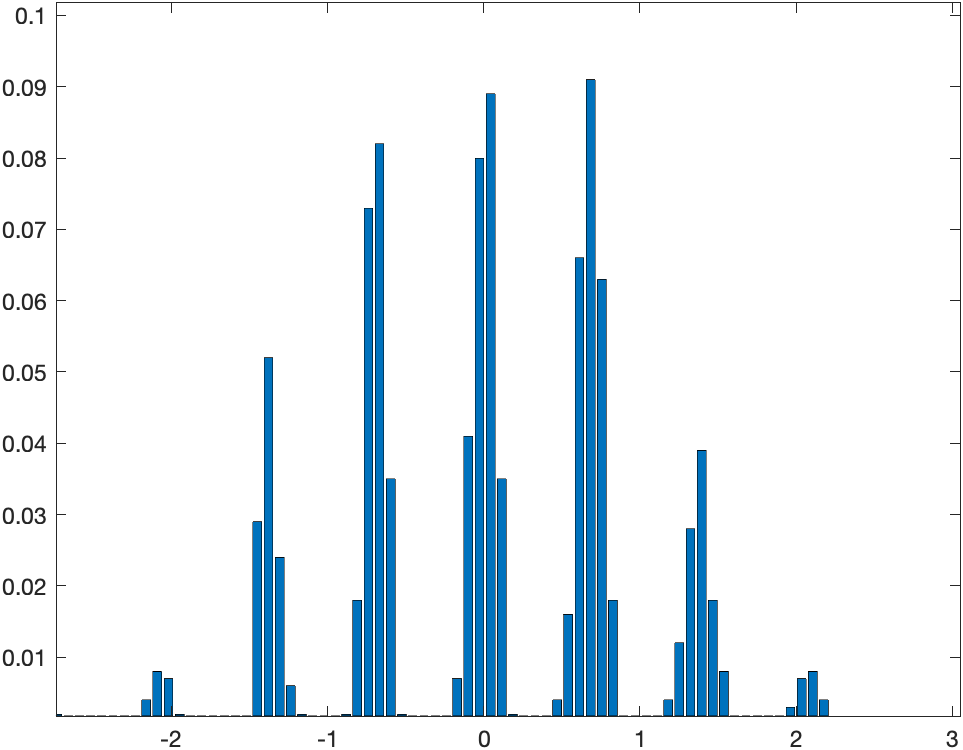
\includegraphics[width=4.3cm]{6-1.png}
    %\caption{fig1}
    }
    \quad
    \subfigure[$n = 20$]{
    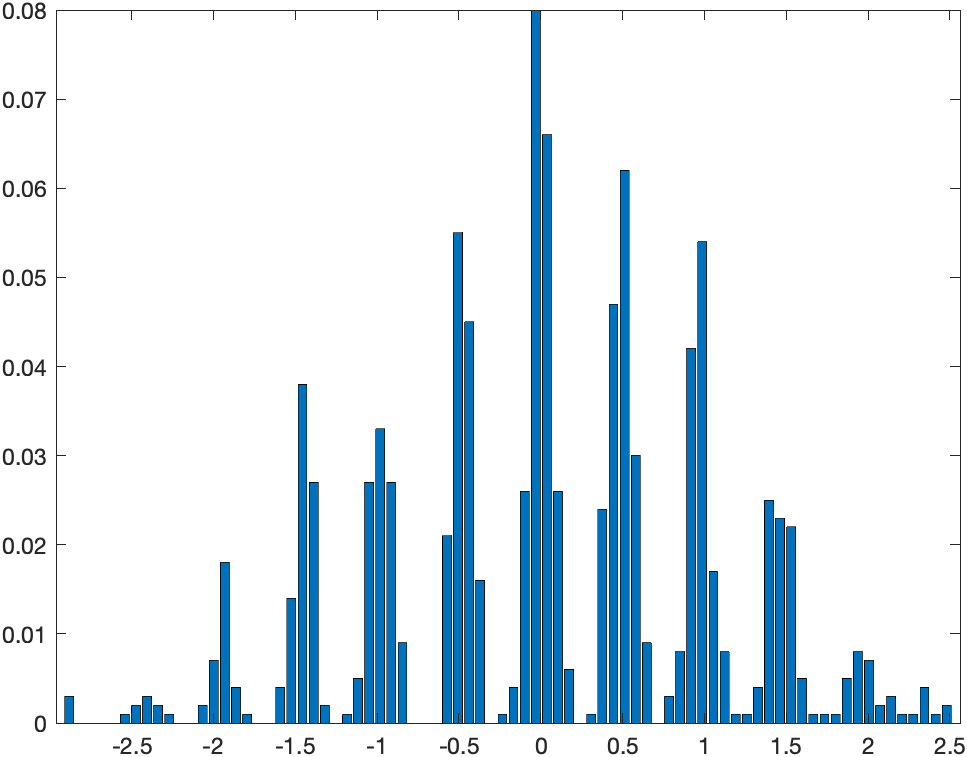
\includegraphics[width=4.3cm]{6-2.png}
    %\caption{fig1}
    }
    \quad
    \subfigure[$n = 50$]{
    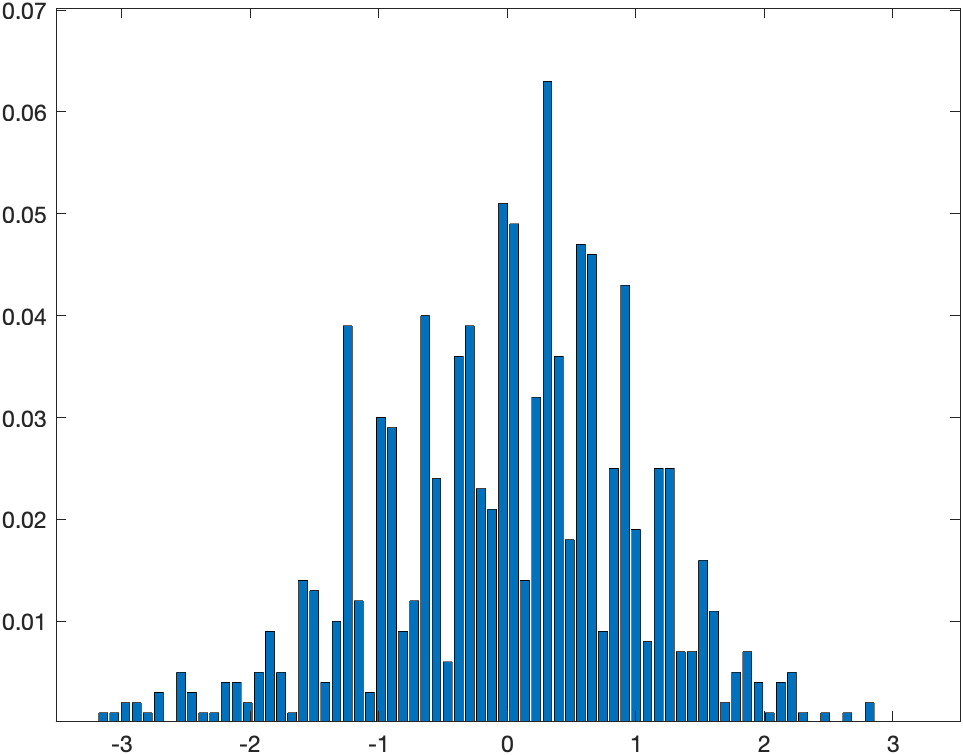
\includegraphics[width=4.3cm]{6-3.png}
    }
    \quad
    \subfigure[$n = 100$]{
    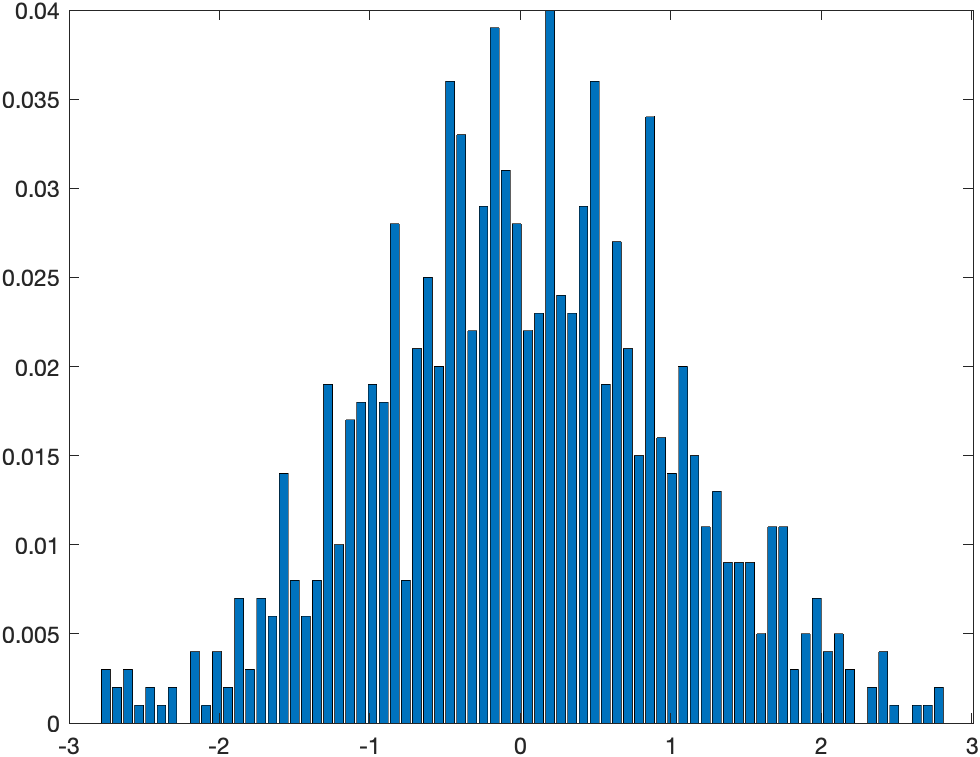
\includegraphics[width=4.3cm]{6-4.png}
    }
    \quad
    \subfigure[$n = 1000$]{
    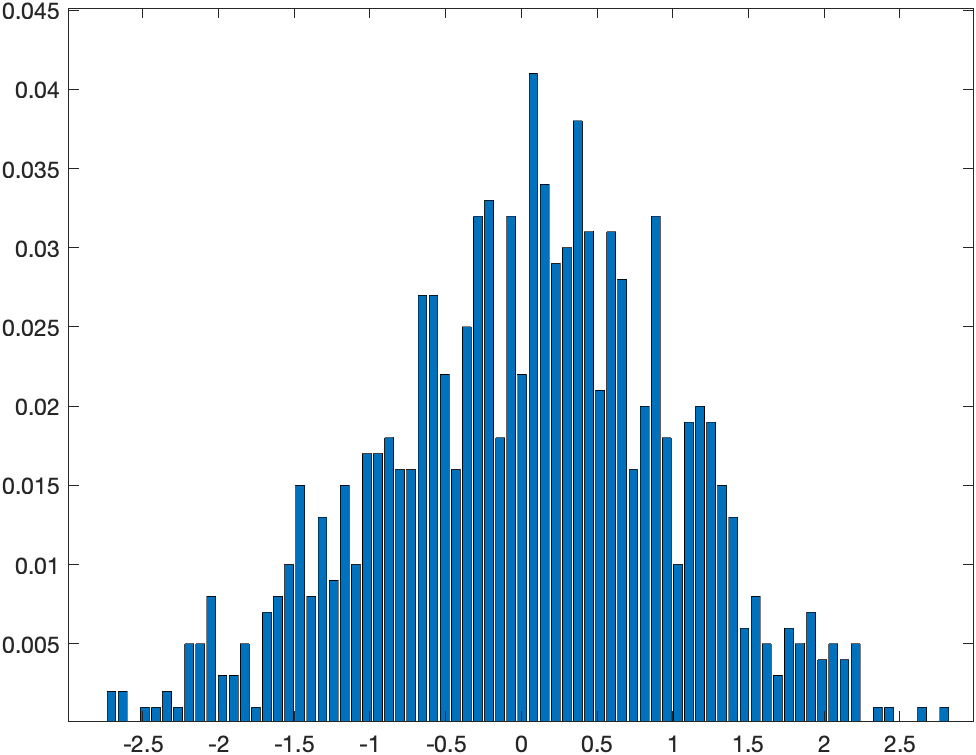
\includegraphics[width=4.3cm]{6-5.png}
    }
    \caption{$\mu_1=0,\sigma_1=2,\mu_2=100,\sigma_2=3, p = 0.7$下,$n$变化时生成的$U_i$的频率分布直方图}
    \label{fig6}
\end{figure}

\subsection{结论和讨论}

\textbf{结论:}当$n$比较小时,频率直方图的“峰”数量较多,且“峰”与“峰”之间间隔较大,随着$n$的增大,“峰”与“峰”之间的间距逐渐变小。同时随着$n$的增大,$U_i$的分布逐渐趋向于标准正态分布。

\textbf{讨论:}当$|\mu_2|$较小时,频率直方图的峰之间距离较小,使得原本便近似于正态分布,因此改变$n$的取值并不能得到很好的效果。但是当$|\mu_2|$很大的情况下时,若$n$很小,频率直方图峰间距较大,使其与正态分布存在偏差,若$n$很大,根据 Lindeberg-L\'{e}vy 中心极限定理,其分布应近似于标准正态分布。而结果恰恰与标准正态分布相符合。成功验证了 Lindeberg-L\'{e}vy 中心极限定理。

\section{总结与体悟}

通过这次对混合高斯分布相关问题的讨论和实践,我对混合高斯分布中各参数的地位、作用和影响有了更深层次的理解,对其图像和性质有了较好的把我;通过 matlab 生成对应的分布分布,让我具体理解了 Monte-Carlo method 和计算机仿真模拟在概率统计中的重要作用;通过对混合高斯分布的讨论,还进而验证了 Lindeberg-L\'{e}vy 中心极限定理,让我明白了其实际体现。总之,此次探索和讨论让我对概率统计问题的研究方法有所涉猎,更加理解概率密度函数在现实中的表现,还提高了我的计算机编程能力和论文撰写能力。

\section{致谢}

感谢熊德文老师的认真授课和点拨启发。

感谢助教对本次大作业付出的辛劳。

感谢方泓杰同学在 Latex 版式上提供的帮助。

\begin{thebibliography}{1}
\bibitem{bib2}
上海交通大学数学系.《概率论与数理统计》.上海交通大学出版社.2011
\end{thebibliography}


\end{document}
